\chapter{Method}
\label{chapter:secorder}

In this chapter, a methodology employing the Compositional Conditional Diffusion Model (CCDM) is proposed, exploring its application in generating defects for new components. Initially, an extensive dataset from industrial production is utilized, categorized into normal and defective samples, and further classified based on different component types. Subsequently, the model is trained through four key stages.

Section 3.1 involves the labeling of defect types and component group names, providing the model with embeddings formed by concatenating conditions (defect types) and component groups. The image features of component group \(X\), compositional condition embeddings \(C\), and time steps \(t\) are then input into the Unet\cite{Unet} of the Diffusion model\cite{nonequilibrium}. In Section 3.2, the overall architecture of the Compositional Conditional Diffusion Model(CCDM) is presented, demonstrating the fusion of compositional condition embeddings with the image features of defective components. Section 3.3 illustrates the forward process and diffusion process formulas of the CCDM. It also describes how Defect types and Component Groups are transformed from classes to embeddings. Time embedding is introduced into the Resblock\cite{Resblock} of U-Net, allowing time steps to be added to the image features. This aids U-Net in gradually denoising the Gaussian noise matrix during the diffusion process. Importantly, each predicted noise is guided by concatenated embeddings and time steps, directing the removal of random noise from the stochastic Gaussian noise matrix.

Finally, a series of experiments is conducted to verify the model's capability to generate defects for previously unseen components. Additionally, optimizations and improvements are applied to enhance the model's performance and applicability.
\newpage

 
\section{Labeling and Regrouping}
In this study, we undertook the intricate process of data regrouping, aiming to classify components based on their similarities. The primary objective was to group components with subtle differences together, whilst recognizing instances where certain components exhibited exceptionally high degrees of similarity. Simultaneously, we became aware that achieving accuracy in fine-grained classification within this task is an independent and challenging area.

Considering these circumstances, we initially utilized a model pre-trained with MobileNetV3\cite{mobilenetv3} to automate the classification process. However, the outcomes generated by the model did not align with our expectations. Subsequently, we decided to incorporate human judgment in conjunction with the assistance of the model to label components. This hybrid approach, combining automated classification with human expertise, was adopted to enhance the precision and reliability of the labeling process, acknowledging the unique challenges posed by the intricate nature of the task.

\subsection{Observer Consensus Process}
To ensure consistent categorization/grouping, we invited multiple observers to conduct similarity assessments. These observers evaluated the similarity between components through shared guidelines and standardized interpretations. Such a consensus process helped eliminate subjective errors and increased the reliability of the grouping results. 
\subsection{Presentation of Grouping Results}
The grouping results are presented in Figure 3.1, illustrating the restructured component groups. Each group represents the outcome of the observer consensus process, and components within each group are considered similar or related for the reader to comprehend the basis of these groupings. 
\begin{figure}[H]
    \centering
    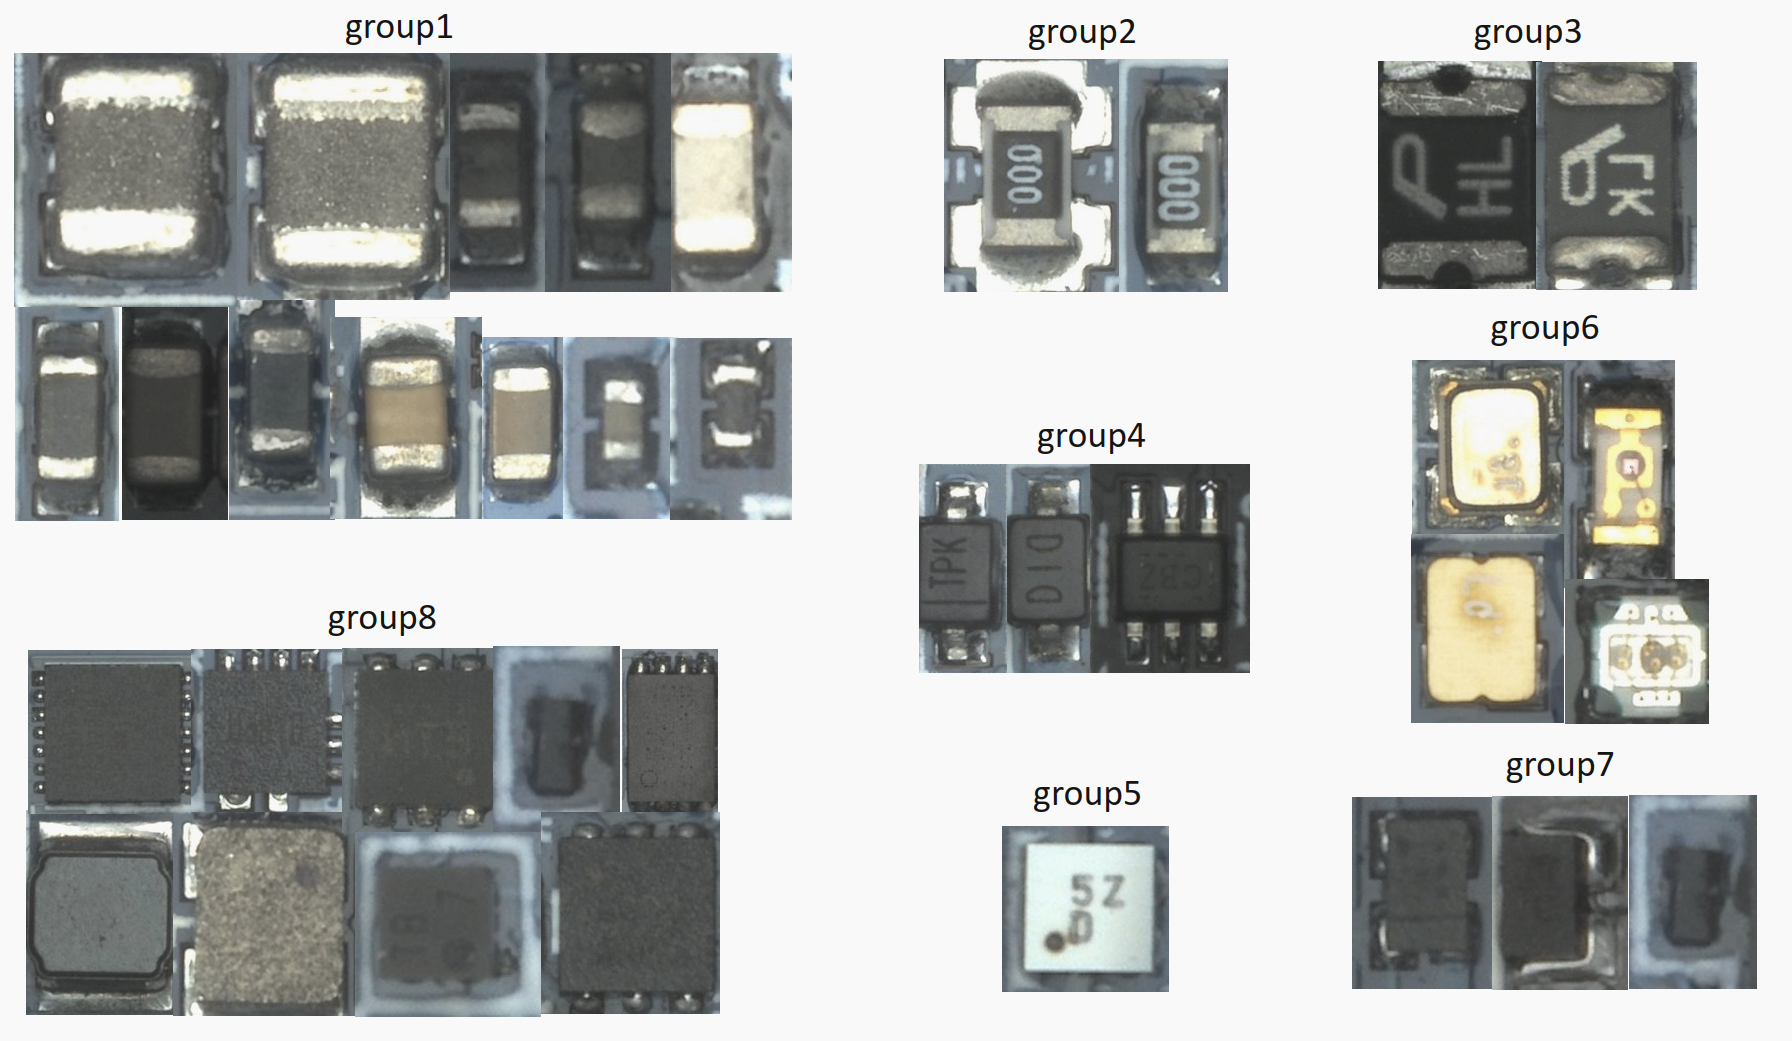
\includegraphics[width=1\linewidth]{Regrouping.png}
    \caption{Presentation of Grouping Results}
    \label{fig:enter-label}
\end{figure}
\section{Model Architectures}
 In this context, we introduce our proposed CCDM in this chapter to generate images of previously unseen defects in new components, as illustrated in Figure 3-2. 
\begin{figure}[H]
    \centering
    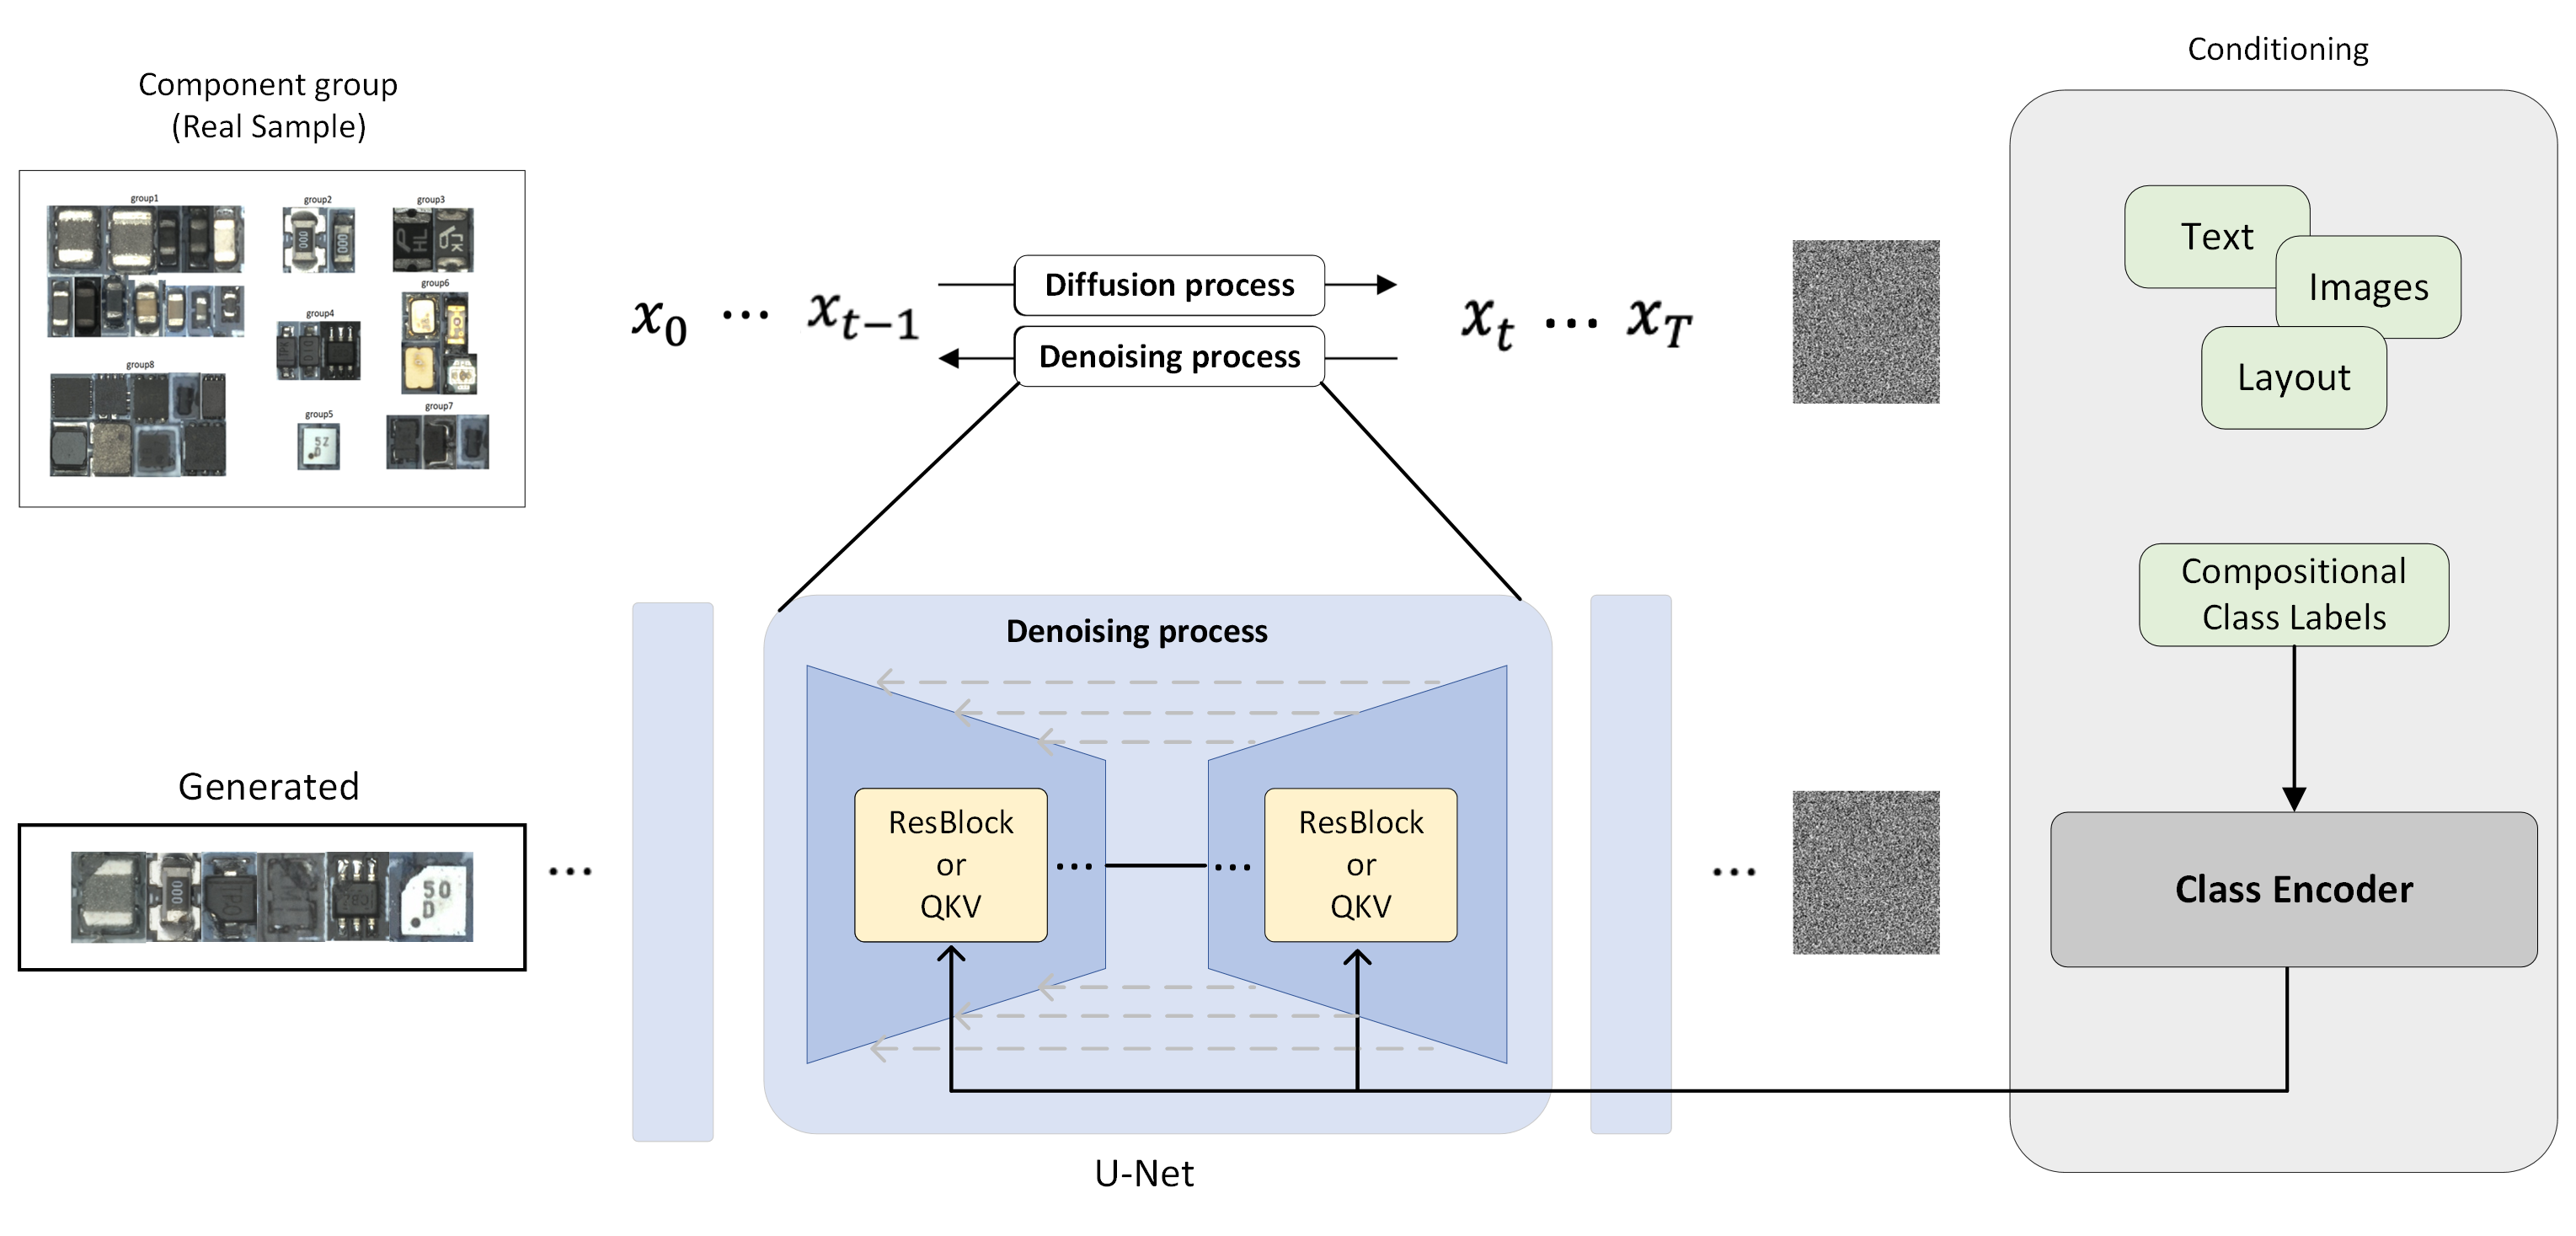
\includegraphics[width=1\linewidth]{Conditional Diffusion model.png}
    \caption{Compositional Conditional Diffusion Model(CCDM)}
    \label{fig:enter-label}
\end{figure}


\section{Conditional Diffusion Model}
Denoising Diffusion Probabilistic Models (DDPM)\cite{DDPM} constitute a class of highly effective generative models in unconditional image generation. DDPM a learned Markov chain to transform a simple distribution, such as an isotropic Gaussian distribution, into the target data distribution. The generative process of DDPM involves learning the inverse process of the forward (diffusion) process a fixed Markov chain gradually adds noise to latent variables \(x_1, ..., x_T\) sampled sequentially from the same dimensions.

In this context, let us consider having a sample  \(x_0\) from the distribution \(D(x|c)\), where \(c\) serves as the compositional condition. The compositional condition \(c\) exhibits variability, and in this study, \(c\) is characterized by the amalgamation of attribute embedding and object embedding, denoted as \(c \in \text{concatenate}(\text{c_{obj}}, \text{c_{atr}})\). This labeling approach signifies the integration of these two embeddings.Here, each step in the forward process is a Gaussian translation. 

\begin{equation}
q(x_t | x_{t-1}, c) := \mathcal{N} (x_t \,|\, c; \sqrt{1 - \beta_t} x_{t-1} \,|\, c, \beta_t I)
\end{equation}



In this process, a fixed schedule of variances, denoted as \( \beta_1, \ldots, \beta_T \), is utilized instead of learned parameters. The procedure involves obtaining \( x_t \) by introducing a small Gaussian noise to the latent variable. Given an initial clean data point \( x_0 \), the sampling of \( x_t \) can be explicitly expressed in a closed form.
\begin{equation}
q(x_t | x_{0}, c) := \mathcal{N} (x_t \,|\, c; \sqrt{\bar{\alpha_t}} x_{0} \,|\, c, (1 - \bar{\alpha_t}) I)
\end{equation}
where $\alpha_t$:= 1 - $\beta_t$ and $\bar{\alpha_t}$ := $\prod_{s=1}^{t}$ $\alpha_s$.
Then a conditional U-Net $\epsilon_{\theta}(x, t, c)$ is trained to approximate the reverse denoising process,
\begin{equation}
p_{\theta}(x_{t-1} | x_t, c) := \mathcal{N} (x_{t-1} \,;\, \mu_{\theta}(x_{t}, t, c); \Sigma_{\theta}(x_{t}, t, c))
\end{equation}
The variance \(\mu_{\sigma}\) can be learnable parameters or a fixed set of scalars. As for the mean, after reparameterization with \(x_{t} = \sqrt{\bar\alpha_{t}}x_{0} + \sqrt{1 - \bar\alpha_{t}}\epsilon\)  for $\epsilon\sim$ $\mathcal{N} (0, I)$, the loss function can be simplified as:
\begin{equation}
L := \mathbb{E}_{x_0,\epsilon}\||\epsilon - \epsilon_{\theta}(\sqrt{\bar{\alpha}_t}x_0 + \sqrt{1 - \bar{\alpha}_t}\epsilon, t, c)||
\end{equation}
To incorporate the binary condition \(c\)into the U-Net architecture, we adopt a strategy inspired by\cite{classifierfree}. This involves employing an embedding projection function, denoted as $e$ = $f(c)$, where $f \in \mathbb{R} → \mathbb{R}^n$, and n represents the embedding dimension. Subsequently, the condition embedding is added to feature maps across every Resblocks\cite{BeatGAN}. Following the training of the denoising model, empirical evidence demonstrates that the network is capable of generating the desired conditional distribution $D(x|c)$ given the compositional condition $c$.

Our objective is to derive a segmentation mask from samples generated through a few reverse Markov steps using DDIM \cite{DDIM}. The rationale behind choosing DDIM lies in its capability to deterministically generate a sample \(x_{t-1}\) from \(x_t\) by eliminating the random noise term.
\begin{equation}
x_{t-1}(x_{t}, t, c) = \sqrt{\bar\alpha_{t-1}}\frac{(x_{t} - \sqrt{1-\bar\alpha_{t}}\hat{\epsilon}(x_{t},c)}{\sqrt{\bar\alpha_{t}}}+\sqrt{1-\bar\alpha_{t-1}}\hat{\epsilon_{\theta}}(x_{t},c)
\end{equation}


\subsection{Conditioning Mechanisms}
In principle, diffusion models model conditional distributions in the form of \(D(x|c)\). To achieve this, we implement a conditional denoising autoencoder, denoted as \(\epsilon_{\theta}(x_t, t, c)\), enabling control over the synthesis process through the input \(c\). The widely recognized diffusion models the Stable Diffusion Model\cite{Stable_Diffusion}, known for its effectiveness in general scenarios. However, our focus extends beyond generating images commonly found in everyday life; we target electronic components used in industrial settings. Additionally, our research is to systematically synthesize images of electronic components based on their compositional the application of advanced generative models in the realm of industrial image synthesis.

Furthermore, we aim to pioneer exploration in the underdeveloped domain of Compositional Class-to-Image approaches. To realize this, we adopt a Class Encoding method for encoding the attributes of electronic components (e.g., "Good," "Broke," etc.) and the group names of electronic components, with grouping strategies outlined in Chapter 3.1. 

\textbf{Object conditions(Groups)} : Object conditions refer to specifications that dictate the content of generated images, representing the appearance or category of the desired objects. While CLIP (Contrastive Language-Image Pre-Training)\cite{CLIP} has been widely employed in natural language processing, it faces limitations in handling out-of-vocabulary (OOV) words in the context of text-to-image generation for industrial electronic components. To address this challenge, we draw inspiration from the Stable Diffusion model and make refinements in encoding object conditions. The generation process for object conditions can be described as follows:
\begin{equation}
c_{obj} = \text{Proj}(\text{Emb}(\text{Encoder}(obj)))
\end{equation}

\textbf{Attribute conditions(Defect type)} : Specifically designed for the Defect Type in electronic components, it captures the unique appearance and characteristics of specific component damages. In simpler terms, the Attribute condition reflects the Defect Type of the component. The generation process of the Attribute Condition can be expressed as:

\begin{equation}
c_{atr} = \text{Proj}(\text{Emb}(\text{Encoder}(atr)))
\end{equation}

These two encoded representations are subsequently embedded, as depicted in Figure 3.3. Following this, the embedded vectors are concatenated to yield a unified embedding. Lastly, utilizing an condition mechanism, this combined embedding is mapped to the ResBlock and integrated with timesteps within the U-Net.

\begin{figure}[h]
    \centering
    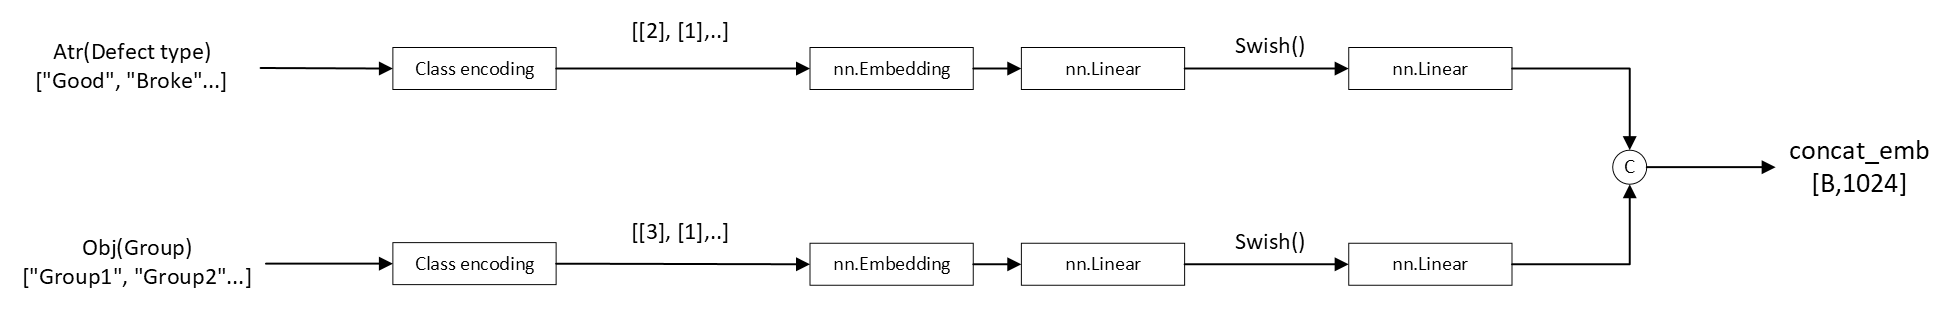
\includegraphics[width=1\linewidth]{Condition_Module.png}
    \caption{Condition Module}
    \label{fig:enter-label}
\end{figure}



\subsection{U-Net}
We also experiment with a layer that we refer to as addition group normalization (AddGN), which incorporates the timestep and class embedding into each residual block after a group normalization\cite{group_normalization} operation. We define this layer as $ \text{AddGN}(h, y) = y_s + \text{GroupNorm}(h) $, where $ h $ is the intermediate activations of the residual block following the first convolution, and $ y = [y_s] $ is obtained from a linear projection of the timestep and class embedding.

\begin{sidewaysfigure}[hp]
    \centering
    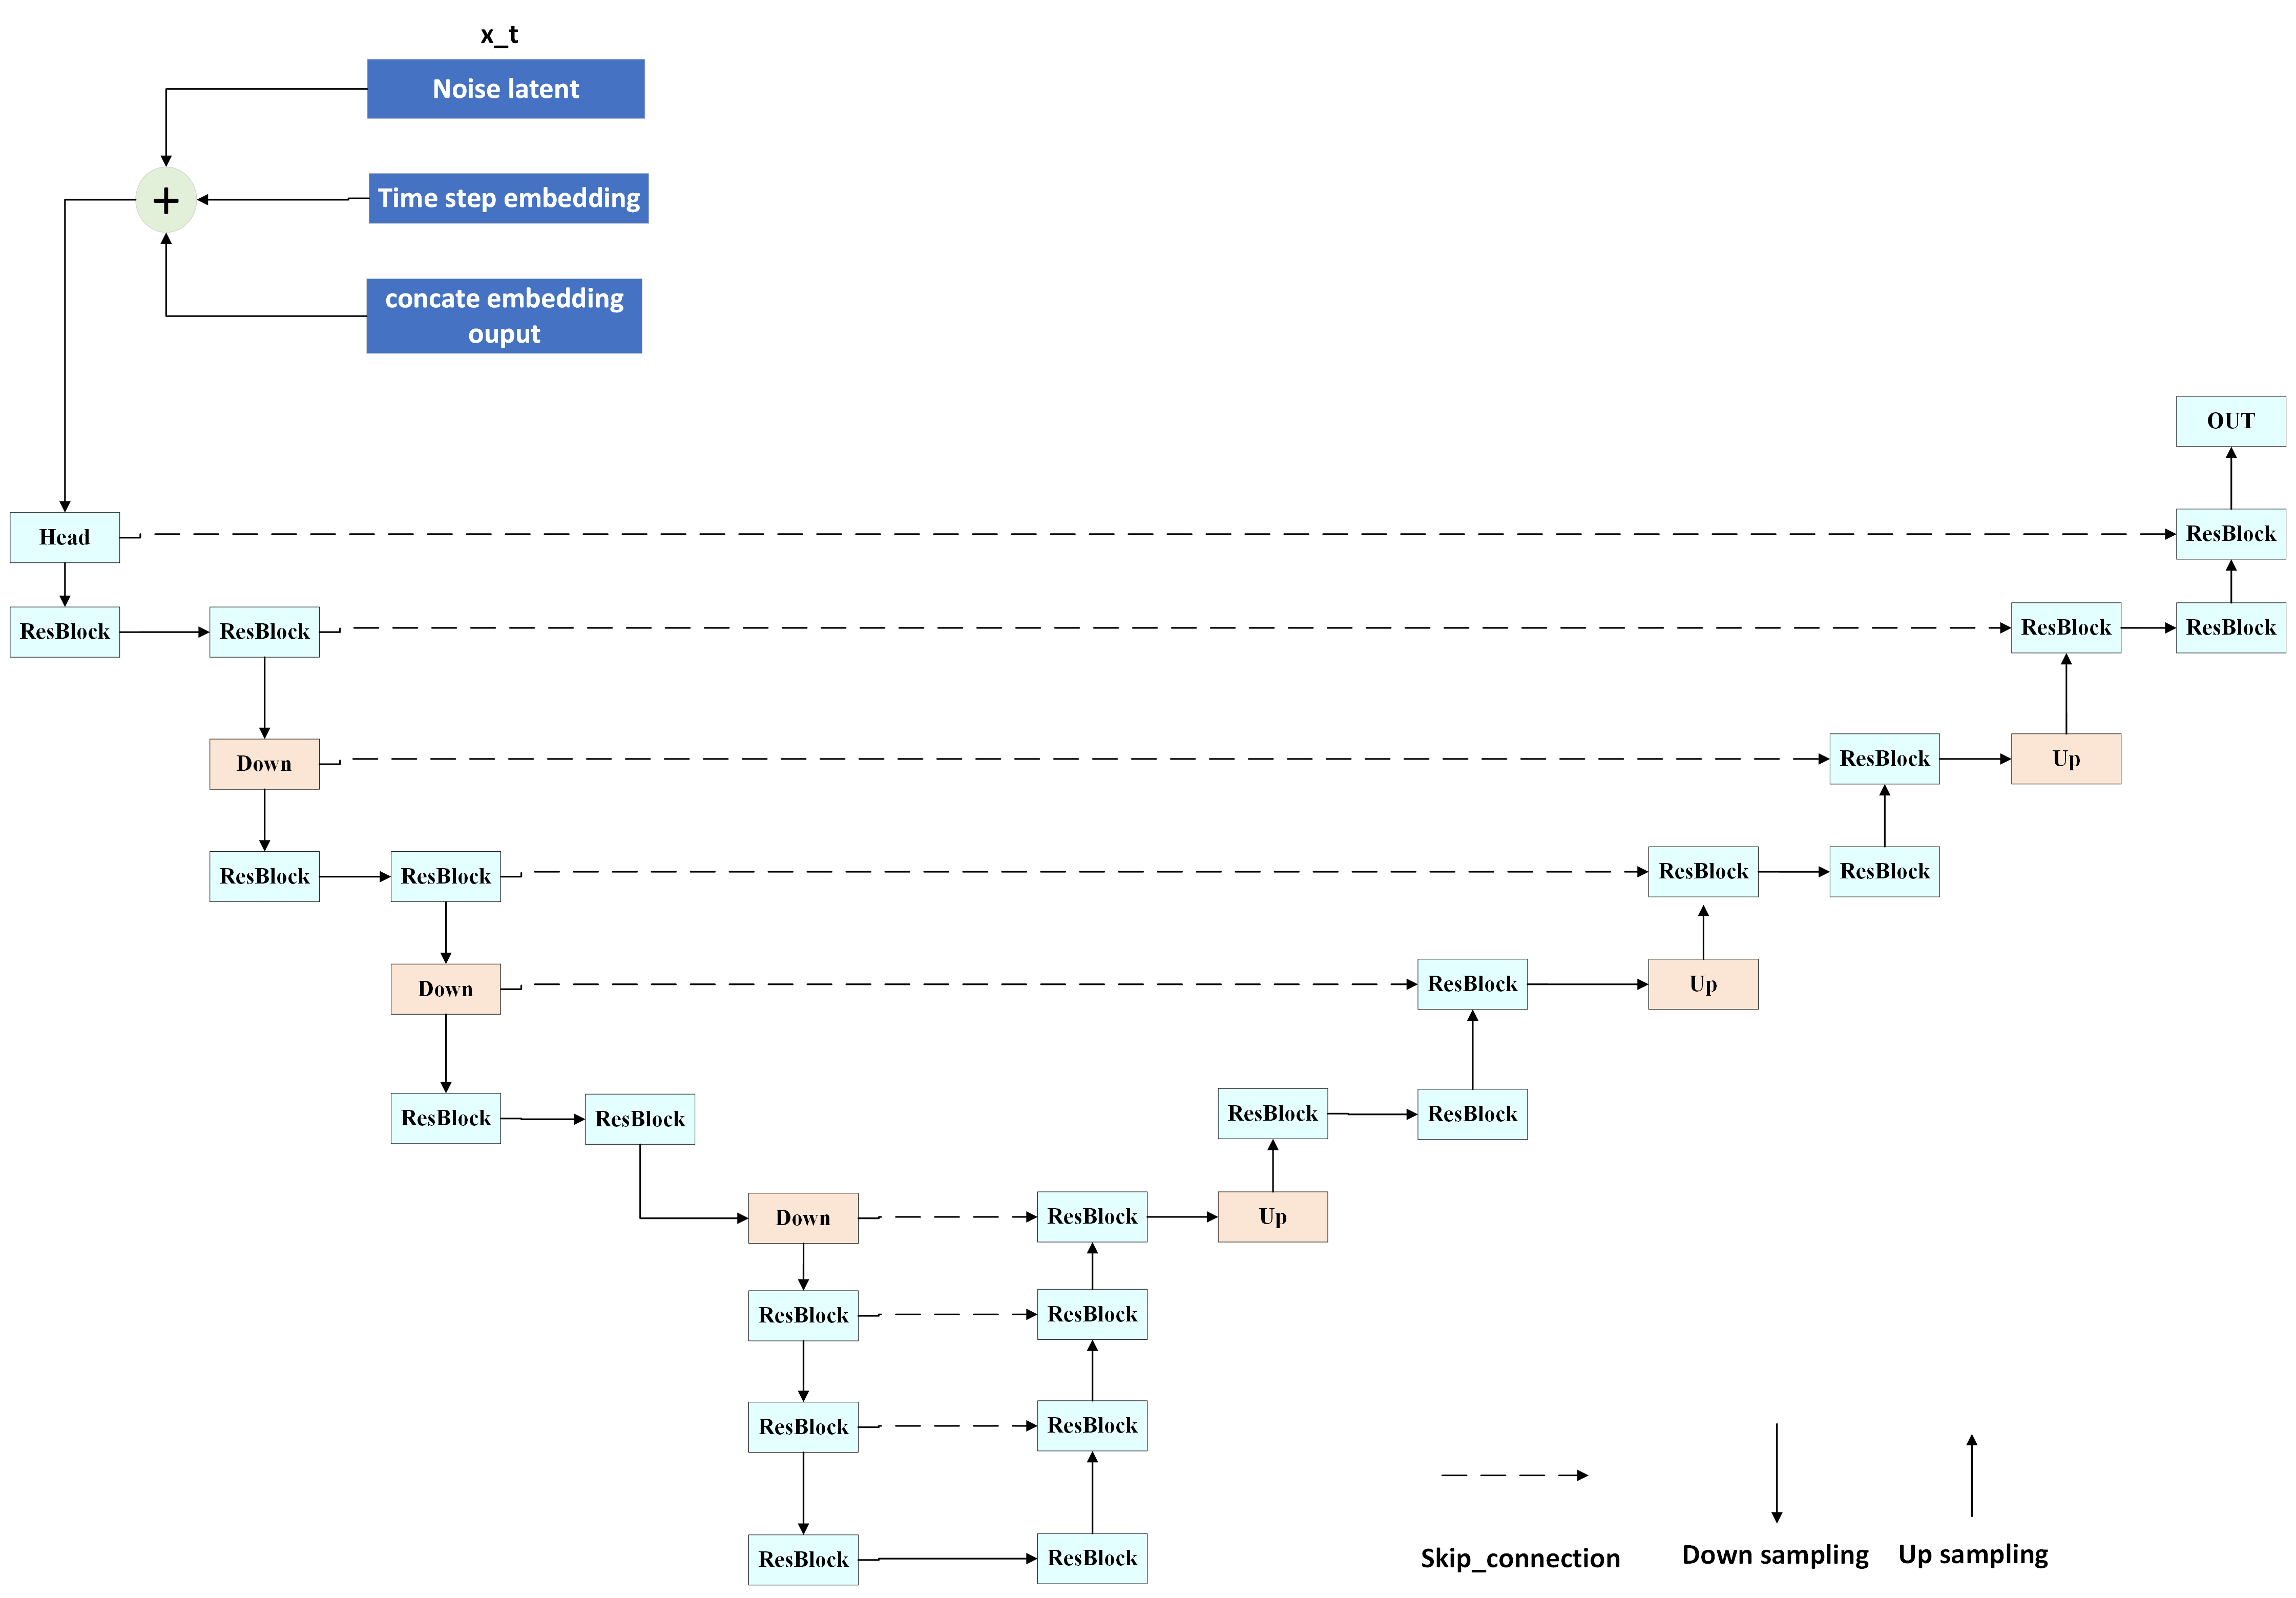
\includegraphics[height=!,width=0.95\linewidth,keepaspectratio=true]{Unet_adaGN.png}
    \caption{U-Net condition mechanisms(U-Net 1)}
    \label{fig:enter-label}
\end{sidewaysfigure}

\newpage
\section{Algorithm}
In the previous sections, we introduced the methods design for our Compositional Conditional Diffusion model,including Conditional Diffusion model, Conditioning Mechanisms, and U-Net condition mechanisms. In this section, we will present the combination of all these methods.
The pseudocode for the proposed Compositional Class-to-image Diffusion model is shown in Algorithm 3.1 and 3.2.

\begin{algorithm}[H]
\caption{Training a diffusion model with classifier-free guidance}
\label{alg:Training}
\begin{algorithmic}[1]
\Statex \hspace{-\algorithmicindent} \textbf{Require:} \(p_{uncond}\): probability of unconditional training
\State \textbf{repeat}
\State \hspace{1em} \((x_0, c) \sim q(x_0, c)\) 
\State \hspace{1em} \(c \leftarrow \emptyset \) \text{with probability} \(p_{uncond}\)
\State \hspace{1em} \(\epsilon \sim \mathcal{N} (0, I)\)
\State \hspace{1em} \(x_t = \sqrt{\bar\alpha_t}x_0 + \sqrt{(1 - \bar\alpha_{t})}\epsilon\)
\State \hspace{1em}Take gradient descent step on \(\nabla_{\theta}||\epsilon_{\theta}(x_t,c,t))-\epsilon||^2\)
\State \textbf{Until} converged
\end{algorithmic}
\end{algorithm}

The algorithm denoted as 3.1 in this research pertains to the training procedure. It involves iteratively sampling from a standard Gaussian distribution to obtain a noise term, denoted as \(\epsilon\). This epsilon is then combined with an initial image \(x_0\) through a forward process, resulting in a noisy image \(x_t\). Subsequently, the generated noisy image \(x_t\), along with a conditioning variable \(c\), is fed into the model to predict the associated noise. The primary objective of the training process is to minimize the disparity between the predicted noise and the actual noise added during the generation process. 

\begin{algorithm}[H]
\caption{Sampling}
\label{alg:Sampling}
\begin{algorithmic}[1]
\Statex \hspace{-\algorithmicindent} \textbf{Require:} \(w\): probability of unconditional training
\State \(x_{T}\sim\mathcal{N} (0, I)\), \(c \sim \)\(p(c)\)
\For{t = T, \ldots, 1}
    \State \(z\sim\mathcal{N}(0, I)\)if \(t > 1,\)else z = 0
    \State \(\tilde\epsilon_\theta = (w + 1)\epsilon_\theta(x_{t},c,t) - w\epsilon_{\theta}(x_t, t)\)
    \State\(x_{x-1} = \sqrt{\alpha_{t-1}}(\frac{x_t - \sqrt{1 - \alpha_{t}}\tilde\epsilon_\theta}{\sqrt{\alpha_t}})+\sqrt{1 - \alpha_{t - 1} - \sigma_{t}^2}\cdot\tilde\epsilon_\theta+\sigma_t\epsilon_t\)
\EndFor
\State \textbf{return} \(x_{0}\)
\end{algorithmic}
\end{algorithm}
Algorithm 3.2 pertains to the sampling process. To obtain the image \(x_{t-1}\), the reverse process outlined in Equation (3.5) is applied. This involves subtracting the noise predicted by the model from the current image \(x_t\), multiplying by certain coefficients, and ultimately adding a noise term \(z\), We then perform sampling using the following linear combination of the conditional and unconditional score estimates\cite{classifier_free}.
\begin{equation}
\epsilon_\theta = (w + 1)\epsilon_\theta(x_{t},c,t) - w\epsilon_{\theta}(x_t, t)
\end{equation}
By following this procedure, the desired image \(x_{t-1}\) is obtained. This sampling algorithm is integral to the overall framework, enabling the generation of sequential images by iteratively applying the reverse process to generate each successive image in the sequence. The incorporation of model-predicted noise, along with carefully tuned coefficients, ensures the accuracy of the generated images and aligns with the overarching objective of achieving realistic and high-quality image synthesis\cite{image_synthesis}.

\section{Different U-Net Architectures}
In this study, we further explored an alternative architectural design to investigate its performance. The detailed architecture is presented below:

Our inspiration originates from the control of conditions in Stable Diffusion. Initially, they employ a pre-trained Language-Image model known as Contrastive Language-Image Pre-Training (CLIP)\cite{CLIP}. This model learns the relationship between a complete sentence and the image it describes. In other words, during training, given an input sentence, the model becomes proficient in retrieving the most relevant images corresponding to that sentence.

Motivated by this model, we delve into the study of a model that establishes a connection between images and classes based solely on class information. Referred to as cMLIP (Compositional  Multi Label-Image Pre-training) We demonstrate in Figure 3.5, this model is designed to link images and classes.
\begin{figure}[H]
    \centering
    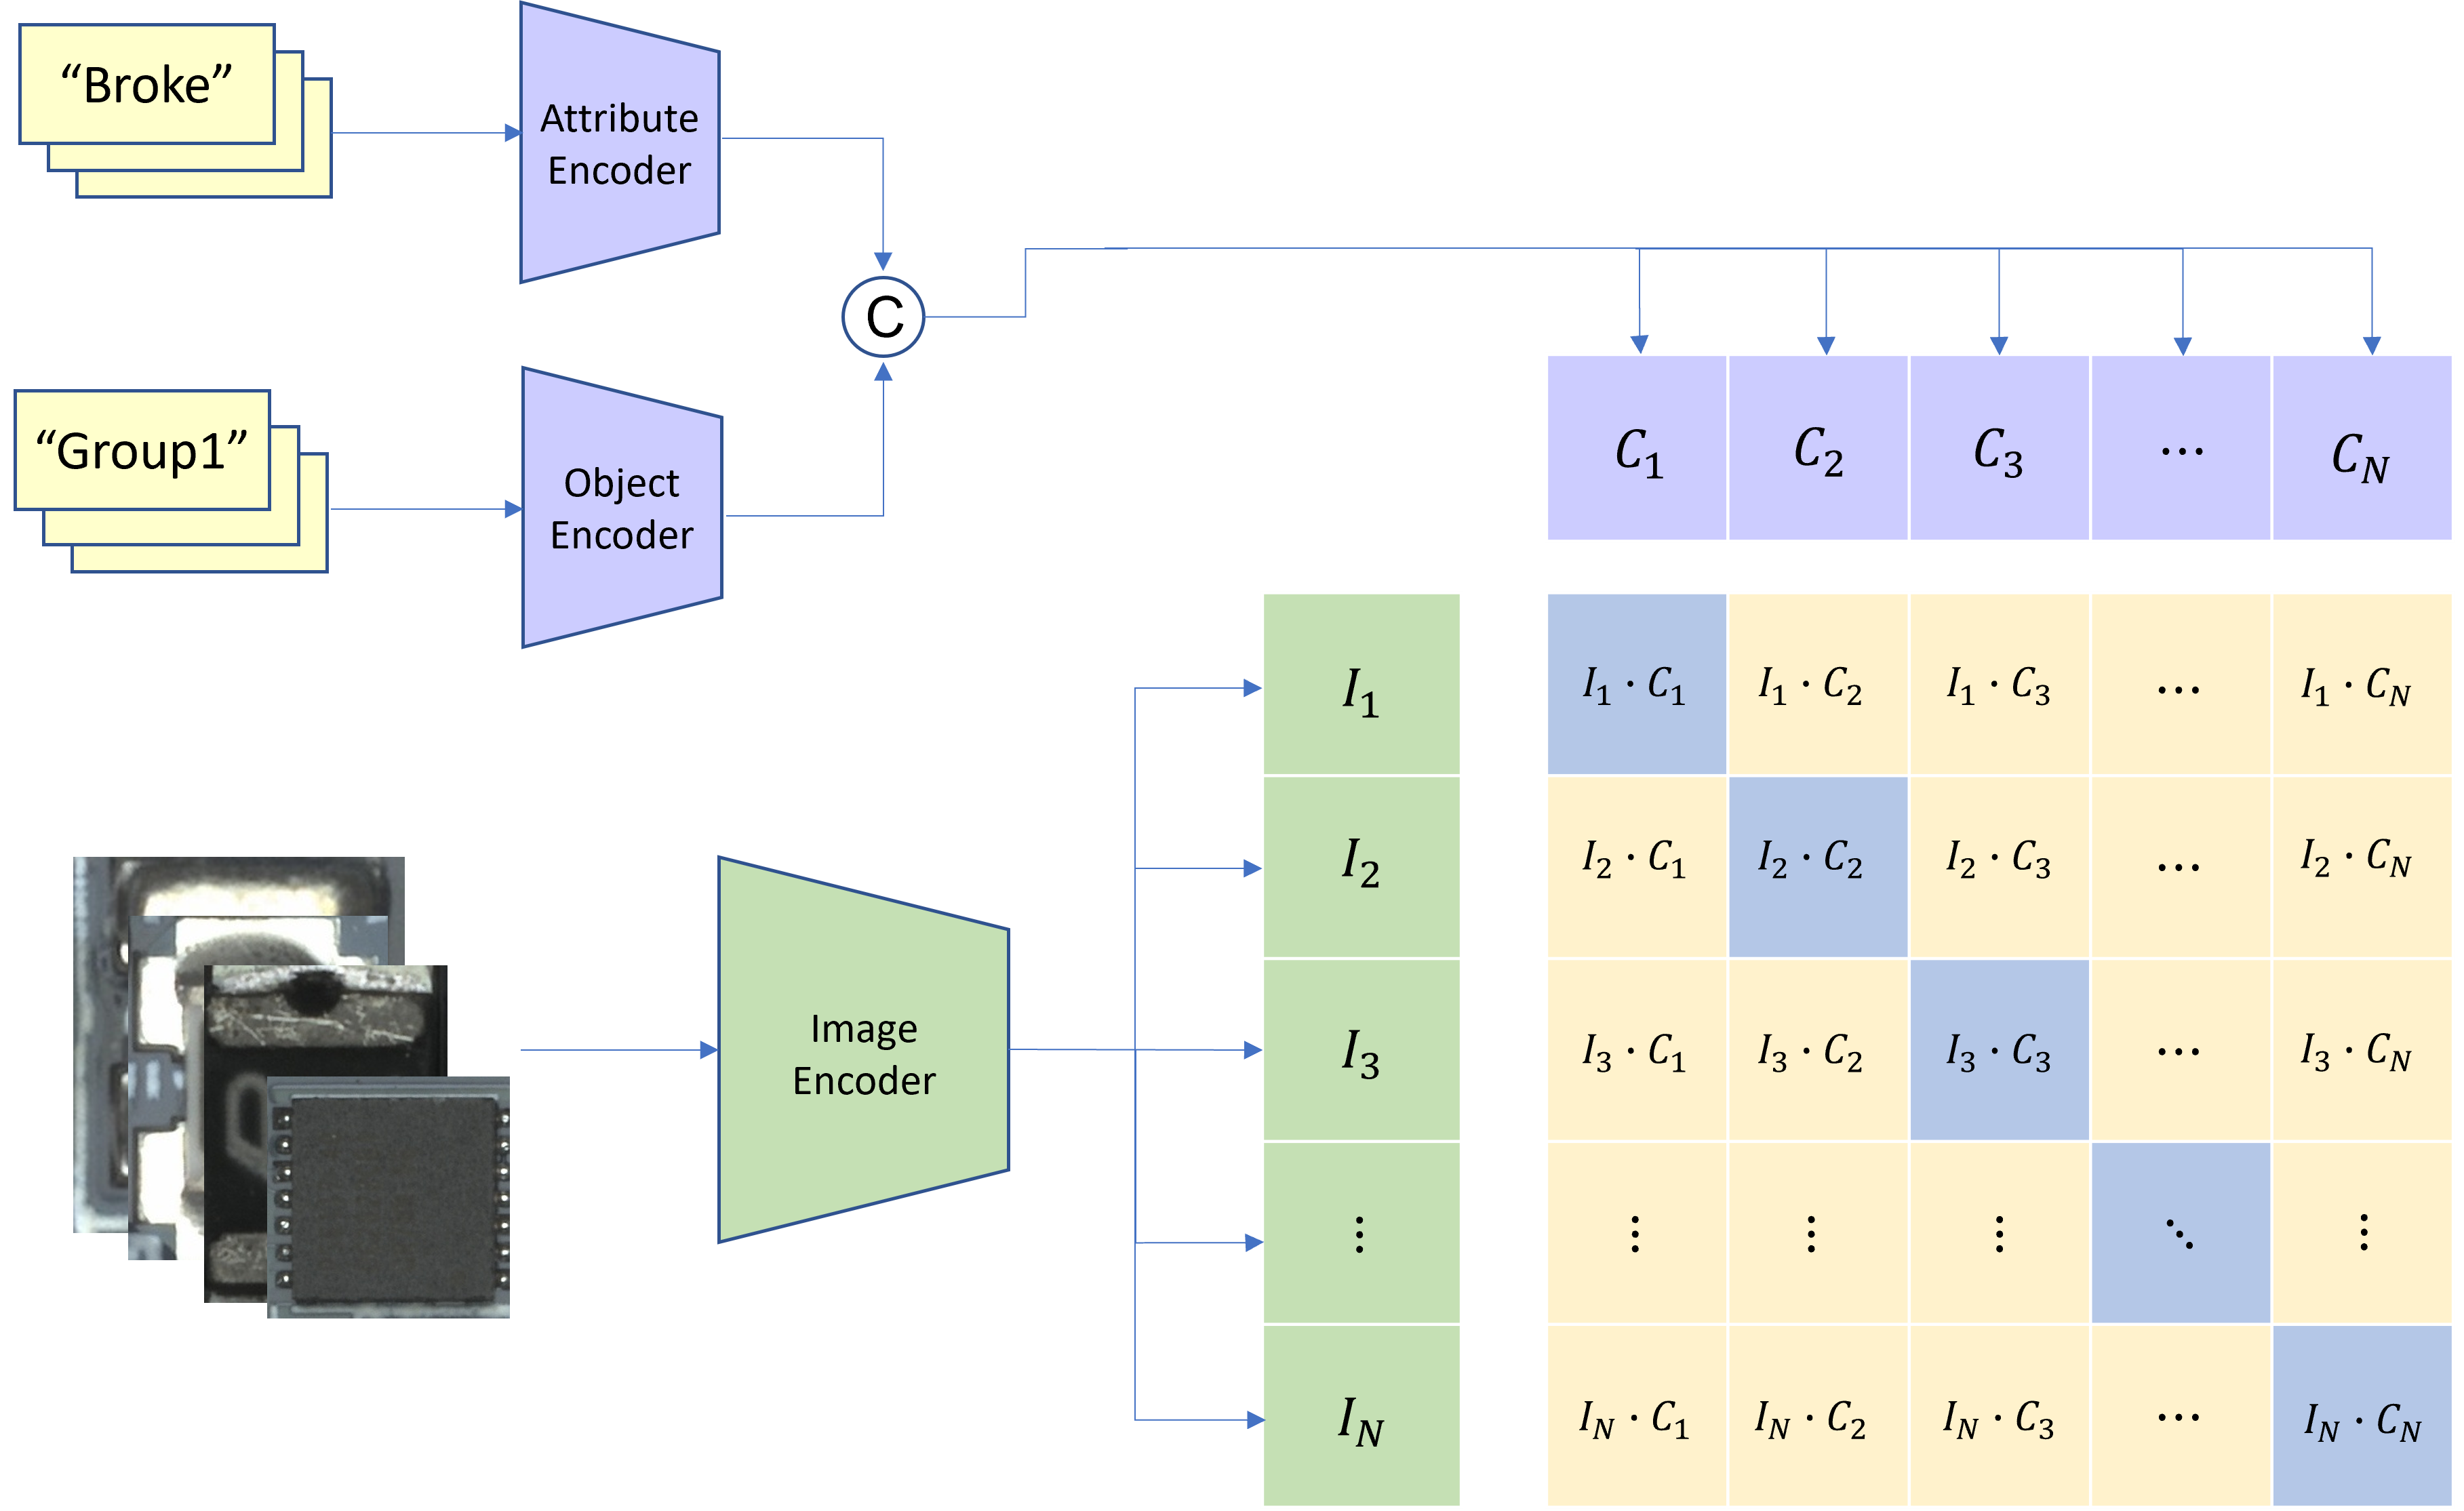
\includegraphics[width=1\linewidth]{cMLIP.png}
    \caption{Contrastive Compositional  Multi Label-Image Pre-training(cMLIP) }
    \label{fig:enter-label}
\end{figure}
Subsequently, we utilize cMLIP in conjunction with a diffusion model to generate images corresponding to specific conditions. This innovative approach draws from the principles of Stable Diffusion and leverages the pre-trained cMLIP model to produce meaningful and self-attention and cross-attention mechanisms, facilitating the fusion of the concatenated embeddings with the Image feature of the defective component condition-controlled image synthesis. Figure 3.6 illustrates the mechanisms of the U-Net with cMLIP.

\begin{sidewaysfigure}[hp]
    \centering
    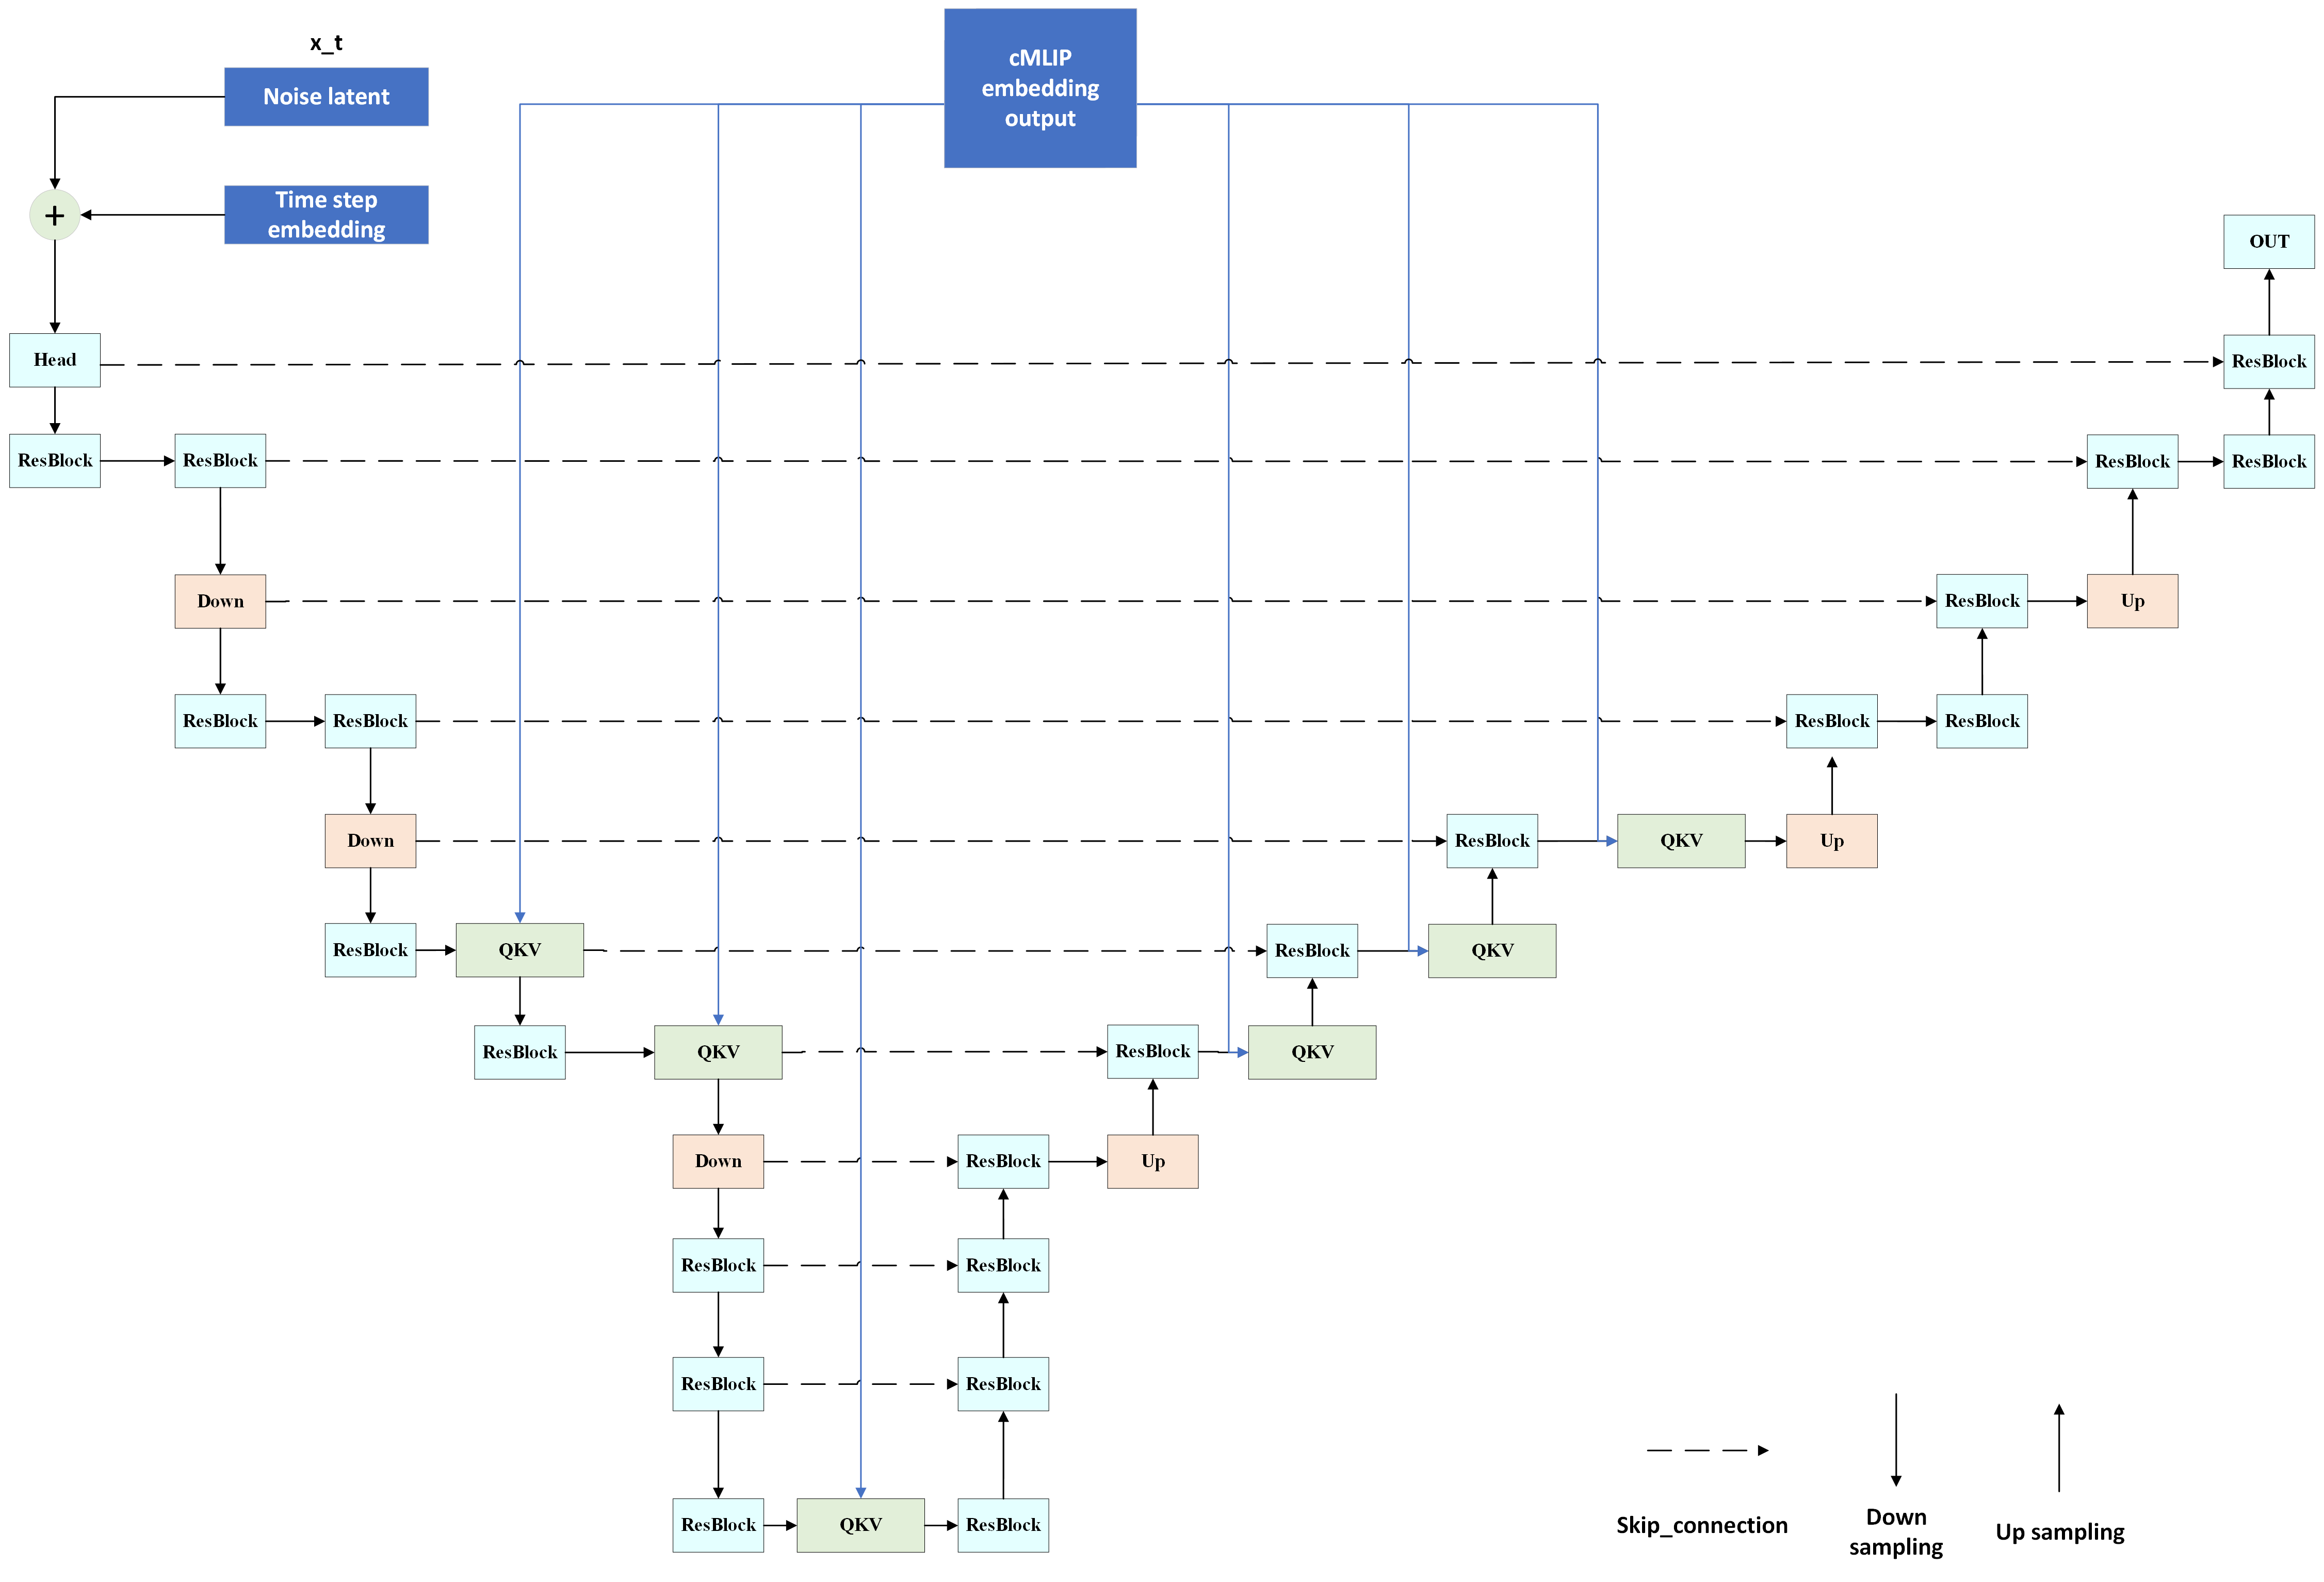
\includegraphics[height=!,width=0.95\linewidth,keepaspectratio=true]{Unet - cMLIP.png}
    \caption{U-Net condition mechanisms(U-Net 2)}
    \label{fig:enter-label}
\end{sidewaysfigure}
\newpage
\section{Select image}
By combining the frameworks mentioned earlier, we can generate relatively indistinguishable unseen images. After producing 50 unseen images (Broke Group3), it was observed that the accuracy of the generated images is not consistently high, with some exhibiting variations in conditions. Consequently, we designed a simple binary classifier using ResNet18 as the backbone to distinguish between "defective" and "non-defective" images. Afterwords, the generated images are fed into this binary classifier for categorization. More precisely, images generated by CCDM are separated, and the classifier is applied to identify "defective unseen images" chosen through this process. This methodology aims to improve the accuracy of generated images and contributes to enhancing the overall effectiveness of the specify what approach in generating realistic and defect-specific unseen images.

